%% Using LaTeX-Boilerplate by Adrian-Tudor Panescu %%
%% https://github.com/adrianp/latex-boilerplate %%

\documentclass[12pt,a4paper,twoside]{report}

\def\pdfshellescape{1} % for epstopdf


\usepackage[utf8]{inputenc}
\usepackage[british]{babel}

\usepackage{algorithm}  % in texlive-science
\usepackage{algorithmic}
\usepackage{amsfonts}
\usepackage{amsmath}
\usepackage{amssymb}
\usepackage{appendix}
\usepackage{caption}
\usepackage{listings}
\usepackage[left=2cm,right=2cm,top=2cm,bottom=2cm]{geometry}
\usepackage{graphicx}
\usepackage{hyperref}
\usepackage{makeidx}
\usepackage{placeins}
\usepackage{subcaption}

\usepackage{epstopdf}  % load after graphic[s,x]


%% bold float labels
\DeclareCaptionLabelFormat{myformat}{\textbf{#1}~\textbf{#2}}
\captionsetup{labelformat=myformat}

%% detailled margin sizes
%\addtolength{\textwidth}{4cm}
%\addtolength{\oddsidemargin}{-1.5cm}
%\addtolength{\evensidemargin}{-1.5cm}
%\addtolength{\textheight}{4.5cm}
%\addtolength{\topmargin}{-3cm}
%\setlength{\parindent}{0pt}
%\setlength{\parskip}{1ex}

%% Section number format
\renewcommand*\thesection{\arabic{section}}

%% Give numbers to subsubsections and add them to index
\setcounter{secnumdepth}{3}
\setcounter{tocdepth}{3}

% rename abstract with care for babel package
\addto\captionsbritish{%
  \renewcommand{\abstractname}%
  {Summary}%
}

%% rename index with care for babel package
\addto\captionsbritish{%
  \renewcommand{\contentsname}%
  {Table of Contents}%
}

%% special table cell that allows line breaks
\newcommand{\specialcell}[2][l]{%
  \begin{tabular}[#1]{@{}c@{}}#2\end{tabular}}

%% do not split long footnotes over multiple pages
\interfootnotelinepenalty=10000


\author{
    Adrian-Tudor Panescu \\
    \href{mailto:adrian@panescu.com}{adrian@panescu.com}
  \and
    John Doe
}
\title{LaTeX Boilerplate}
\date{}  % no date


\begin{document}

  \maketitle

  % blank pages are inserted for two-side printing
  %!TEX root=../main.tex

\thispagestyle{empty}
%\addtocounter{page}{-1} % do not count this page
\newpage
\mbox{}
\pagebreak


  \setcounter{page}{3}

  \begin{abstract}
    Lorem ipsum dolor sit amet, consectetur adipiscing elit. Duis rutrum, arcu quis venenatis porta, sapien massa feugiat elit, ac malesuada arcu tortor vitae lacus. Phasellus quam urna, condimentum at mollis eu, vehicula dictum velit. Nulla facilisi. Sed neque dolor, posuere in nibh in, lacinia blandit risus. Duis sed nisi at lorem suscipit condimentum nec ut mi. Vivamus dictum metus ut nisi fringilla, feugiat hendrerit augue sollicitudin. Sed malesuada diam ac eros interdum pellentesque. Praesent sed laoreet nibh, vitae sodales ipsum. Pellentesque a congue dui, posuere adipiscing enim. Nulla facilisi. Nulla augue ipsum, pellentesque eu sapien in, facilisis consectetur leo.

Vivamus in urna commodo dui ornare ornare. Nulla facilisi. Curabitur sodales interdum porta. Proin hendrerit sem ac neque molestie, sit amet viverra leo malesuada. Nulla imperdiet sit amet neque in fringilla. Vestibulum vehicula elementum magna, sit amet sagittis velit tristique a. Nam feugiat magna quam, quis aliquet ante lacinia sed. Duis ut nisl eu leo faucibus tincidunt vel sit amet mauris. Phasellus consectetur elit tempor nisi hendrerit, ut dapibus nibh faucibus. Aenean in tellus nisl. Integer elementum, quam facilisis tempus fermentum, neque augue consectetur diam, nec sodales neque sem non lacus. Pellentesque feugiat libero metus, in fermentum lorem dictum at. Proin.
  \end{abstract}

  \tableofcontents
  \listoffigures
  \listoftables
  \lstlistoflistings

  % next page will be odd-numbered (assumes \FloatBarrier)
  \cleardoublepage

  \section{Introduction}
    \label{sec:intro}
    Thank you for chosing LaTeX-Boilerplate \cite{ref:latex-boilerplate}!


  \cleardoublepage

  \section{Examples}
    \label{sec:ex}
    This section exemplifies some useful elements.

    \FloatBarrier

    \subsection{Algorithm}
      \label{sec:algo}
      Here is an example of an\footnote{algorithm \ref{alg:fizz}.}

\begin{algorithm}{$FizzBuzz(n)$}
    \caption{FizzBuzz}
    \label{alg:fizz}
    \begin{algorithmic}[2]
        \FOR{$i \gets 1; i \le n; i \gets i+1$}
            \IF{$i$ is divisible by $15$}            
                \STATE{output FizzBuzz}
            \ELSIF{$i$ is divisible by $3$}
                \STATE{output Fizz}
            \ELSIF{$i$ is divisible by $5$}
                \STATE{output Buzz}
            \ELSE
                \STATE{output i}  
            \ENDIF
        \ENDFOR
    \end{algorithmic}
\end{algorithm}

    \clearpage

    \subsection{Listing}
      \label{sec:lst}
      %!TEX root=../../main.tex

This sections exemplifies a source code listing \ref{lst:lst}.

\vspace*{1\baselineskip}

\begin{figure}[!ht]
\lstinputlisting[language=Python,
                 frame=tb,
                 captionpos=b,
                 numbers=left,
                 showspaces=false,
                 showstringspaces=false,
                 showtabs=false,
                 stepnumber=2,
                 numbersep=4pt]
  {static/lst/fizzbuzz.py}
  \caption{Python 3 implementation of the Fizz Buzz game.}
  \label{lst:lst}
\end{figure}


    \clearpage

    \subsection{Float}
      \label{sec:float}
      %!TEX root=../../../main.tex

This section demonstrates how to insert images in your document.


      \FloatBarrier

      \subsubsection{Figure}
        \label{sec:fig}
        %!TEX root=../../../main.tex

Here is an example of a Figure \ref{fig:fig}.

\begin{figure}[!h]
  \centering
  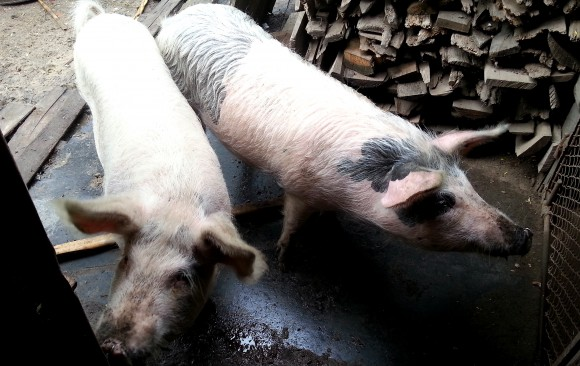
\includegraphics[scale=0.5]{static/img/pigs1.jpg}
  \caption[This is a special label, used only in the List of Figures]
          {Pigs, pigs, pigs.}
  \label{fig:fig}
\end{figure}


      \FloatBarrier

      \subsubsection{Subfigure}
        \label{sec:subfig}
        %!TEX root=../../../main.tex

And here is an example of a float \ref{fig:subex} with subfigures
\ref{fig:subex:pigs} and \ref{fig:subex:pig}.

\begin{figure}[!ht]
  \centering
  \begin{subfigure}[b]{0.3\textwidth}
    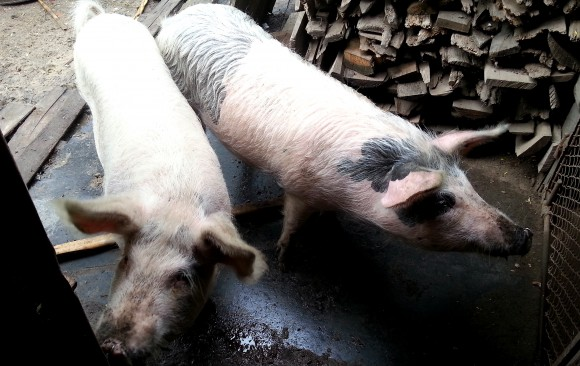
\includegraphics[width=\textwidth]{static/img/pigs1.jpg}
    \caption{Some pigs.}
    \label{fig:subex:pigs}
  \end{subfigure}
  \begin{subfigure}[b]{0.3\textwidth}
    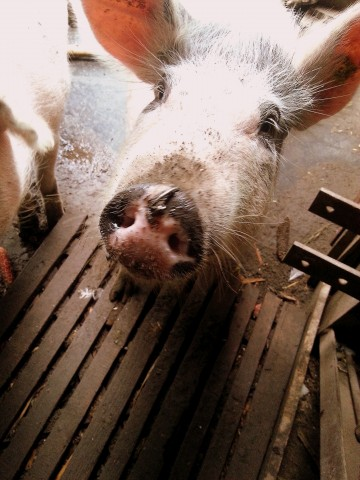
\includegraphics[width=\textwidth]{static/img/pigs2.jpg}
    \caption{A pig.}
    \label{fig:subex:pig}
  \end{subfigure}
  \caption{Some pigs being pigs.}
  \label{fig:subex}
\end{figure}


     \clearpage

    \subsection{Table}
      \label{sec:tbl}
      %!TEX root=../../main.tex

This section exemplifies insertion of tabular data \ref{tbl:tbl}.

\begin{table}[!ht]
  \centering
  \begin{tabular}{| c | c | c | c | c |}
    \hline
    \textbf{Value} & \textbf{Fizz} & \textbf{Buzz} & \specialcell[t]{\textbf{Fizz} \\ \textbf{Buzz}} \\ \hline \hline
    1 & No & No & No \\ \hline
    2 & No & No & No \\ \hline
    3 & Yes & No & No \\ \hline
    4 & No & No & No \\ \hline
    5 & No & Yes & No \\ \hline
    6 & Yes & No & No \\ \hline
    7 & No & No & No \\ \hline
    8 & No & No & No \\ \hline
    9 & Yes & No & No \\ \hline
    10 & No & Yes & No \\ \hline
    11 & No & No & No \\ \hline
    12 & Yes & No & No \\ \hline
    13 & No & No & No \\ \hline
    14 & No & No & No \\ \hline
    15 & Yes & Yes & Yes \\ \hline
  \end{tabular}
  \caption{The FizzBuzz game values.}
  \label{tbl:tbl}
\end{table}


  \cleardoublepage

  \section{Conclusions}
    \label{sec:outro}
    %!TEX root=../../main.tex

That's all folks!


  \nocite{*}  % include uncited references
  \bibliographystyle{plain}
  \bibliography{bib/myrefs}

  \appendixpage
  \addappheadtotoc

  \appendix
    \section{An appendix}
    \label{sec:app}
    %!TEX root=../../main.tex

Lorem ipsum dolor sit amet, consectetur adipiscing elit. Vestibulum
nec nisi non dui accumsan dignissim eu in lacus. Pellentesque vel
enim dolor. Mauris condimentum velit dolor, a ultrices purus commodo
in. Etiam malesuada justo libero, vel accumsan est commodo in. Donec
eleifend risus non massa dapibus, sit amet bibendum nibh viverra.
Duis non quam vehicula, fringilla nisi ut, interdum libero. Etiam vel
neque aliquam, suscipit enim ut, laoreet leo.

Aliquam erat volutpat. Cras in lorem mauris. Nunc vel sapien
pharetra, sollicitudin est vitae, auctor ligula. Sed sagittis rutrum
feugiat. Nulla semper, urna sit amet feugiat tincidunt, mauris tellus
egestas dolor, et tempor odio nibh sit amet diam. Quisque eget
ullamcorper odio, in imperdiet nisi. Curabitur varius at libero nec
sollicitudin.

Donec sed est ac lacus lobortis sollicitudin. Morbi dui mi, suscipit
eget pretium sit amet, sollicitudin consectetur purus. Quisque
tincidunt ornare tellus, id tincidunt quam euismod nec. Sed rutrum
mauris non lorem elementum porttitor. Quisque dignissim et diam sit
amet convallis. Nulla sed tellus lobortis sapien tincidunt bibendum.
Phasellus cursus mi diam, vel vestibulum urna consequat eu.
Pellentesque vestibulum, risus a tincidunt pulvinar, tellus mi
vestibulum nulla, non cursus lectus eros ac mi. Duis sollicitudin
mauris massa, malesuada posuere diam tincidunt et. Pellentesque
volutpat ligula sed dolor auctor, nec volutpat enim suscipit. Duis a
metus magna. Vestibulum id turpis ac urna dictum lobortis. Cras
semper sem nec sem dapibus sodales.

Pellentesque convallis a tortor nec tempus. Donec nec varius lectus.
Quisque vel rhoncus nulla, nec ultricies purus. Nulla eget velit
diam. Sed eu sapien sed arcu euismod auctor volutpat sit amet sapien.
Aenean orci eros, ultrices et urna quis, consectetur convallis dolor.
Vestibulum ante ipsum primis in faucibus orci luctus et ultrices
posuere cubilia Curae; Nulla lectus dolor, feugiat vel augue non,
molestie posuere odio. Donec placerat elementum lacus, id auctor eros
commodo id. Sed at blandit tellus.

Nulla nibh massa, porttitor quis blandit dignissim, consectetur at
augue. Vestibulum id sagittis ligula, ac consequat diam. Nunc vel
nunc a tortor porttitor tempus eget at elit. Integer lacinia orci at
suscipit suscipit. Mauris vehicula pulvinar lectus, id posuere orci
semper quis. Nullam porta, sem ac luctus consequat, lectus mi
vulputate dui, id egestas ante massa cursus lorem. Cras a dictum
quam, eu scelerisque justo. Donec id mattis tortor. Proin sodales
ligula quis nisi tempor condimentum. Fusce tincidunt mattis justo.
Curabitur sit amet tortor quam. Maecenas dignissim velit at purus
commodo congue non vitae lacus.


\end{document}
